\documentclass[9pt,twocolumn]{scrartcl}

\usepackage{ucs}
\usepackage[utf8x]{inputenc}
\usepackage[T1]{fontenc}
\usepackage[english]{babel}

%\usepackage{graphics}%	images other than eps

\usepackage[paper=a4paper,top=2cm,left=1.5cm,right=1.5cm,bottom=2cm,foot=1cm]{geometry}

\usepackage{relsize}%	relative font sizes

\usepackage[retainorgcmds]{IEEEtrantools}%	IEEEeqnarray

\usepackage{epstopdf}
\usepackage{indentfirst}
\usepackage{hyperref}
\usepackage{graphicx}
\usepackage{listings}
\usepackage{color}

%%%%%%%%%%%%%%%%
%  title page  %
%%%%%%%%%%%%%%%%
\titlehead{University of Minho \hfill Master's Degree in Informatics Engineering\\	Department of Informatics \hfill Parallel and Distributed Computing}

\title{Profiling + CUDA}

\subtitle{A finite volume case study from an industrial application}

\author{Miguel Palhas \hfill--- \texttt{\smaller pg19808@alunos.uminho.pt}\\Pedro Costa \hfill--- \texttt{\smaller pg19830@alunos.uminho.pt}\\\smaller Stéphan Clain (co-Advisor)\\
}

\date{Braga, February 2012}

\subject{Integrated Project}


%%%%%%%%%%%
%  Hacks  %
%%%%%%%%%%%

%	Paragraph with linebreak
\newcommand{\paragraphh}[1]{\paragraph{#1\hfill}\hfill

}


\begin{document}
\maketitle

\begin{abstract}
Two parallelization approaches, one using shared memory with OpenMP, and another using a GPU running CUDA code, were implementend, and later profiled and analysed, to understand the scalability of this options for a scientific application. The case study was a two dimensional Finite Volume problem that simulates the propagation of a pollutant in a given environment. The results of the analysis will provide insight on how to approach this kind of problems, how to identify potential bottlenecks, and evaluate the scalability of a parallelized code against the original version.
\end{abstract}

\section{Introduction}
This document analyzes an application which computes the evolution of a pollutant in a given environment, studying possibilities of optimization and/or parallelization.\\

The application calculates the pollutant spread area at variable moments during a given time interval. This pollutant spreads according to a partial differential equation which is solved using the Finite Volume Method.\\

The algorithm used by the program loops until the specified time interval is reached. At each iteration of this main loop, the flux of pollution is calculated in each edge (performed by a function named \texttt{compute\_flux}) and the mesh pollution levels are updated (performed by the \texttt{update} function).\\

Two attempts of parallelization are intended: one using shared memory on a multiprocessor system and one using a GPU.\\

The final aim is to have a qualitative and quantitive comparison of both versions against each other and the original sequential code, and an evaluation of possible bottlenecks and/or optimizable code parts.\\

%\subsection{Structure}% what will we do (list of actions), a.k.a. structure
An initial profiling of the application, including the methodology and conclusions, is presented in \autoref{sec:initprof}. In \autoref{sec:optm&para}, the initial profiling information is used to identify the parts of the algorithm/code which are better suited for optimization and/or parallelization. The implementation of a shared memory parallel version and a GPU version are explained, profiled and analyzed in \autoref{sec:openmp}  and \autoref{sec:cuda}, respectively. A comparison of the results obtained for each implementation is performed in \autoref{sec:comparison}.\\

\section{Sequential}% why did we choose compute_flux & update to mess with
\label{sec:initprof}
The analysis of the sequential code starts with the generation of it's callgraph, from which it is possible to find the function where the program execution spends most of it's time. According to Amdahl's Law, the speedup to get from parallelization will be directly limited by how big the parallelizable code fraction is. Therefore, this function should be the first to study for optimizations and/or parallelization, as it's where one can profit the most from speedup.\\

For the purpose of generating the call graphs throughout this document, the \texttt{Callgrind} tool\footnote{From the Valgrind suite.} was used. The information generated by this tool could then be visualized using \texttt{KCachegrind}.\\

Originally this reported 11\% of the execution time in the \texttt{compute\_flux} function and 8\% in the \texttt{update}, while the remaining\footnote{A very small percentage of the time is spent on other functions, which can therefore be ignored} 80\% of the time was spent with I/O (to build an animation). Since the goal is to optimize the computation, the I/O calls were removed and the profiling tool reported 63\% of the time in the \texttt{compute\_flux} and the remaining time in the \texttt{update} function. This results are shown in \autoref{fig:callgraph.orig.anim} and \autoref{fig:callgraph.orig.still}.\\

\begin{figure*}[!htp]
	\begin{center}
		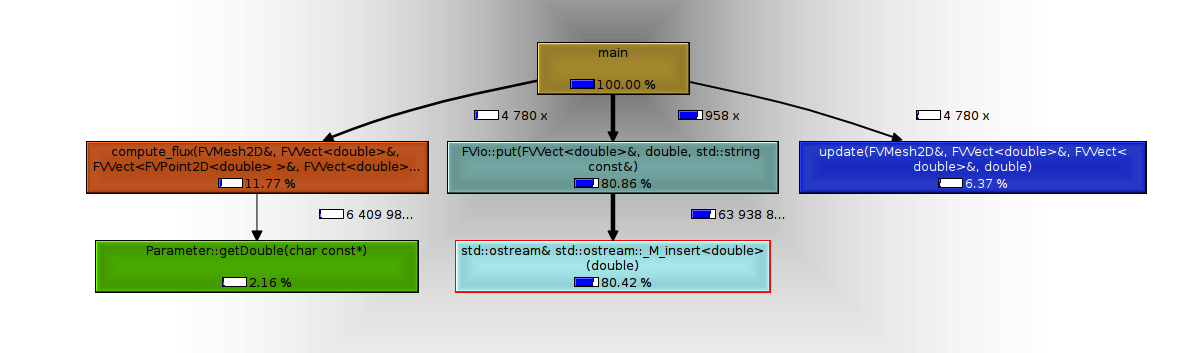
\includegraphics[width=\textwidth]{images/output.png}
	\end{center}
	\caption{Callgraph of the original application (with animation).}
	\label{fig:callgraph.orig.anim}
\end{figure*}

\begin{figure*}[!htp]
	\begin{center}
		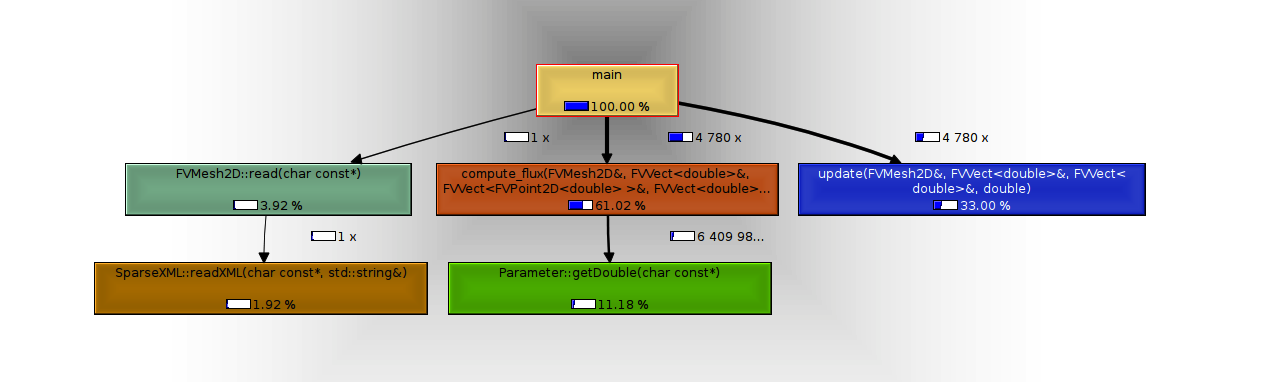
\includegraphics[width=\textwidth]{images/no_output.png}
	\end{center}
	\caption{Callgraph of the original application (without the animation).}
	\label{fig:callgraph.orig.still}
\end{figure*}


\section{Optimization \& Parallelization}
\label{sec:optm&para}
As determined in \autoref{sec:initprof}, the best targets for optimization and/or parallelization are the \texttt{compute\_flux} and \texttt{update} functions, which will be the primary and secondary goals for this project, respectively (each parallelized version will be focusing on these functions by this order).\\

The first optimization possible in the \texttt{compute\_flux} function is the removal of the \texttt{Parameter.getDouble()} call. This was meant to retrieve the Dirichlet condition value from the parameter file, but being this a constant throughout the program execution, the value can be loaded in an early preparation stage and sent as an argument to \texttt{compute\_flux}. Additionally, moving this argument to a global variable can reduce the function call overhead.\\

Excessive dereferencing is a common problem on both functions and is directly related to the FVLib library. Although the usage of pointers may greatly improve code readability, the increased memory accesses caused by deep levels of dereferencing tend to aggravate effects of any memory bottlenecks. With some adjustments to the library internal structures, the same or better readability might be achievable with fewer pointers and lower reference depth. To solve this, the first major change made in each implementation was the definition of new, more efficient structures to improve computation capabilities.\\

Lastly, to allow the parallelization in both intended approaches, the loops themselves have to be changed both in \texttt{compute\_flux} and \texttt{update}. The original code uses a non-standard iterator-like approach to loop through the elements of the mesh. While this works in sequential code, it won't work with conventional parallelization mechanisms, as there would be no knowledge of the iterations other than the data itself (which is not enough). This mechanisms requires index based accesses, or at least random-access iterators\footnote{OpenMP works with both, CUDA works naturally with indexes.}. Since the FVLib library already implements index based accesses, the changes in the loops are trivial.\\

\subsection{Dependencies}
\label{subsec:dependencies}
\subsubsection{\texttt{compute\_flux}}
In the \texttt{compute\_flux} function a data dependency can be found which prevents parallelization. This dependency is found in the calculation of $\Delta t_{i}$ (the final value $\Delta t_{n}$ is returned by the function) and causes each iteration to depend on the previous one (the first iteration uses a preset value $\Delta t_{0}$).\\

Through some mathematical manipulations this calculation can be removed from the loop and the dependency replaced with a calculation of the maximum computed velocity ($v_{max}$), which can be computed through a reduction.\\

The method of calculation through reduction is the best option to parallelize the calculation of iteration dependent associative binary operators ($\sum$,$\prod$,min,max). The goal of this method is to reduce the problem size as the computation advances: each thread picks two values, and in the next step only half the threads are needed, until only one is left with the final value.\\

While most of the original application was designed to allow fully featured models, some simplifications were performed in the actual implementation. Some of these simplifications can be used to further optimize this specific code, thus achieving better results at the expense of already absent features.\\

One of such simplifications is the usage of constant velocity vectors for each cell of the loaded mesh. The original algorithm computes the resultant velocity on each edge, based on the velocities of the adjacent cells. Since this computation relies only on constant data, it's results are also constant, and can be calculated in an early preparation stage of the program. Also, since $\Delta t_{i}$ is calculated using the maximum computed velocity, it will be constant throughout the entire execution, and can, therefore, be precomputed before the main loop starts. This simplifies the \texttt{compute\_flux} algorithm, and completely removes the need for a reduction.\\

\subsubsection{\texttt{update}}
The \texttt{update} function also holds a problem when thinking of parallelization. This function iterates through the edges of the mesh, computes the contribution of each edge to the adjacent cells pollution values, and updates the final value. Since each cell has multiple edges and the final value associated with a cell is the sum of the contributions from all it's edges, then multiple iterations might be changing this value simultaneously.\\

It is possible to remove this dependency by changing the loop itself to iterate over each cell calculating the final value from all it's edges, instead of iterating over the edges. Considering that no edge data is changed, this completely removes the dependency and allows the parallelization of the function.\\

Nevertheless, this is not a perfect scenario due to false sharing: a thread changing a given cell may invalidate a set of contiguous cells in cache, forcing subsequent accesses to take longer. To prevent this, each cell could store the pollution contributions from each of it's edges separately, and the final value would be a sum reduction on each cell, using an accumulator which would most probably stay in a register, successfully preventing false sharing. However, this level of optimizations are out of the scope of this document.\\

\section{OpenMP}
\label{sec:openmp}
\subsection{Implementation}
\subsubsection{Data Structures}
The excessively deep levels of dereferencing used in FVLib hold an obvious performance bottleneck. It causes the processor to spend a lot more time waiting for data than necessary.\\

The first optimization performed in the given application is the implementation of new data structures. These group the data required for the computation according to the object -- cells and edges -- in indexed arrays, this way reducing the dereference levels to the bare minimum. Also, grouping the data of the iterated objects into structures and placing these in contiguous arrays improves locality, allowing more operations to be performed with less memory accesses.\\

\subsubsection{Setup}
As discussed in \autoref{subsec:dependencies}, some adjustments are required in order to parallelize both core functions.\\

Using the new structures, changing the loop in \texttt{update} is a trivial operation. Besides the required change in the structure to be iterated, a change in the internal algorithm is required. In the original version a branch operation is used to handle border edges, where there is only one adjacent cell. This is replaced by another branch that identifies the current cell as either the left or right cell in the scope of an edge. Despite allowing the parallelization, this change implies a trade-off: since both core functions must be executed consecutively and each will iterate on a distinct structure, the data fetched to feed one may cause the data required for the other to be discarded from cache.\\

In order to remove the dependency in the \texttt{compute\_flux} function, the calculation of $\Delta t_{i}$ must be replaced with the calculation of $v_{\mathrm{max}}$ -- the maximum computed velocity -- which can then be calculated through a reduction. The \texttt{max} reduction exists implemented in the OpenMP framework but only since the version 4.7 of \texttt{gcc}, which is not yet the standard at the date of this document. Consequently, this operation was implemented by making each thread calculate it's local maxima (thus effectively removing any race condition), and storing it in an array. After the parallel zone, the array is sequentially scanned to find the global maximum. To prevent false sharing, each thread saves the local maxima in the array only after the loop.\\

As previously stated, in this particular implementation, the $v_{\mathrm{max}}$ computation can be completely moved from \texttt{compute\_flux} to an early preparation stage, as the problem is simplified to consider the velocity vector field constant throughout the entire execution. Although this strips the code of an abstraction layer, it reduces the number of operations performed by \texttt{compute\_flux} without compromising this particular implementation results.\\

\subsubsection{Parallelization}
The main feature about OpenMP that makes it so interesting to create shared memory parallel code is that the program itself is almost equal to the sequential version, with the addition of the required directives and adaptation tweaks (mainly to solve concurrency problems).\\

After applying the OpenMP directives, only one parallelizable loop is left unexplored -- the one used to iterate over the edges of a cell in the \texttt{update} function. This happens due to the maximum number of edges per cell, as defined in the FVLib, being as low as nine and because this would imply increasing the complexity in the structures and the \texttt{update} function's algorithm. This has low optimization potential and the trade-offs have to be tested and studied in order to find if it is worth. As was previously mentioned, this level of optimization is out of this document's scope.\\

Because there are no nested parallel loops in this code, the number of threads to be issued are set by default to the maximum number of threads supported by the hardware to be executing at any given time. Despite that, this number is multiplied by a factor (1 by default) to allow experiences to be easily conducted using more threads. The goal of this approach is to try to achieve an effect similar to the one in GPUs: theoretically, issuing more threads than those the hardware can execute in parallel may improve efficiency by allowing any thread to step in while another is stalled on any resource.\\

To parallelize both \texttt{compute\_flux} and \texttt{update}, a \texttt{parallel for} OpenMP directive is placed in each just before the inner loop. Considering all the variables external to the parallel zone as shared, all the required variables must be explicitly made private (either with the \texttt{private({\textit{list}})} clause or by declaring the variables only inside the parallel zone).\\

\subsection{Profiling}
Considering that the final OpenMP version can be built from the original version with incremental steps (described previously as the optimizations and preparations performed), five versions of the code are analyzed in this section:
\begin{description}
\item[Original]{The original provided application code, only with the required adaptations to the testing environment;}
\item[Structs]{The implementation of new structures to optimize memory accesses;}
\item[Update]{The version with the changed loop iterations in the \texttt{update} function;}
\item[Optimal]{Last optimizations, mostly around the already assumed simplifications of the problem;}
\item[OpenMP]{The parallel shared memory version using OpenMP.}
\end{description}

%%\subsubsection{PAPI framework}% why doesn't PAPI have class in the source FFS
%%To profile the resulting code with some detail, a framework was implemented to take advantage of C++ features (such as exceptions and objects) when using the PAPI library.
%%
%%This framework allows to group several events into predefined sets, as long as creating custom sets on the go. Given the changes required to profile OpenMP code, this framework greatly facilitates the library error handling, improving robustness and readability.
%%
%%The following sets are predefined: CPI (total instructions and cycles), Memory (load and store instructions), Flops/s (floating point operations and total cycles), L1 (first level cache accesses and misses), L2 (same for second level cache), Operational Intensity (RAM bytes accessed and Flops), Instructions Per Byte (RAM bytes accessed and total instructions), Multiplication/Addition Balance (FP total, multiplication and division instructions).
%
%%\subsubsection{Methodology}% scripts are cool, talk about them
%To perform measurements in the parallel code the PAPI library requires some adaptation. Although the library initialization and cleanup can (and should) be performed in the same places as the sequential code, each thread in a parallel zone must handle it's own event set. Additionally, when initializing the library, the thread support must be explicitly activated.
%
%Once in the parallel zone, each thread is responsible for creating it's own event set (either predefined or custom), starting it before the loop begins, stopping it after while collecting the results (which are stored in a shared array, like the local maxima), and removing the event set before the parallel zone ends. Outside, the global maximum computation is measured in the same way, and the final	 results are gathered sequentially.

\subsubsection{Test Cases}
\label{subsubsec:testcases}
A total of five test cases of different sizes are used to profile each version of the code, which are listed in \autoref{tab:testcases}.

\begin{table}[!htp]
	\begin{center}
		\begin{tabular}{|c|c|c|c|}
\hline
\textbf{Name} & \textbf{\# Edges} & \textbf{\# Cells} & \textbf{Size}	\\
\hline
Tiny	 & 3780 & 2435 & 227 KB	\\
Small & 15552 & 10192 & 942 KB	\\
Medium & 64145 & 42406 & 3.82 MB	\\
Big & 257989 & 171275 & 15.38 MB	\\
Huge	 & 1044709 & 695033 & 62.36 MB	\\
\hline
		\end{tabular}
	\end{center}
	\caption{Test cases used, sorted by size.}
	\label{tab:testcases}
\end{table}

The first two cases fit in any last level cache, the Medium case reaches the limits of these caches and the remaining levels fit only in RAM. These sizes were calculated while trying to take into consideration the effectively used data, to keep an abstraction between the implementations -- the actual sizes may change between versions.\\

\subsubsection{Environment}
\label{subsubsec:env}
To correctly profile the multiple versions, including the CUDA versions, the same computation node group in the SeARCH cluster was used. The environments used consisted in a single node, fully reserved, with the following characteristics:
\begin{itemize}
\item{Group 511:
	\begin{itemize}
	\item{$2\times$ AMD Opteron 6174 @ 2.2GHz}
	\item{$12\times$ cores/socket}
	\item{64GB RAM}
	\end{itemize}
	}
\end{itemize}

The roofline model for this particular system can be found in \autoref{fig:roofline.511}. According to \cite{AMD6100} each processor has a theoretical peak of 211 Gflops/s. The processors ceilings were defined based on thread level parallelism, operations balance and data level parallelism, by this order. The peak memory bandwidth of 42.03 GB/s was obtained with the STREAM benchmark. The only ceiling for the memory bandwidth is defined by using only one data channel.\\

\begin{figure}[!htp]
	\begin{center}
		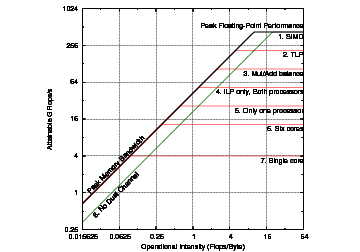
\includegraphics[width=\columnwidth]{images/roofline511}
	\end{center}
	\caption{Roofline of the Group 511 nodes in the SeARCH cluster.}
	\label{fig:roofline.511}
\end{figure}

\subsubsection{Methodology}
In each version, three optional objects were added to measure full, main loop and core functions execution time, respectively. The objects measure the time intervals using the Unix time functions, with precision to the microsecond, and try to take their own overhead into consideration when calculating the results. Storage mechanisms and time arithmetic are done by the predefined Unix functions, to minimize the probability of human error.\\

To minimize interferences, every test is run in a fully reserved computation node, and only one timing object is active in a given execution. Which object is activated is defined at compile time.\\

Despite not being the perfect approach, this mechanisms allow a reasonable comparison given the limited CUDA profiling environment.\\

\subsection{Results}
\label{sec:omp:results}
The most important values to report are the speedups obtained with each performed optimization, which are presented in \autoref{tab:speedups}. To avoid excessive clutter, only the results for the largest test case are shown.\\

\begin{table}[!htp]
	\begin{center}
		\begin{tabular}{|l|cccc|}
\hline
speedups & Full & Main Loop & \texttt{compute\_flux} & \texttt{update}	\\
\hline
Original & 1 & 1 & 1 & 1	\\
Structs & 3.35 & 3.29 & 4.55 & 2.03	\\
Update & 2.78 & 2.77 & 4.53 & 1.71	\\
Optimal & 3.37 & 3.42 & 6.09 & 1.54	\\
OpenMP & 8.33 & 8.50 & 15.75 & 1.52	\\
\hline
		\end{tabular}
	\end{center}
	\caption{Speedups achieved with each optimization and with the parallelization for the Huge test case in a Group 511 computation node.}
	\label{tab:speedups}
\end{table}

Looking at the obtained values the conclusion arises that just by changing the structures used one can easily get noticeable speedups due to a better memory management.\\

The change in the \texttt{update} loop is also to notice. While it allows parallelization, as predicted the change increases execution time due to a need to replace much of the content in the cache levels.\\

Removing the need to compute velocity obviously has a high impact in the \texttt{compute\_flux} function, and compensates the speedup lost before.\\

Lastly, the OpenMP version gets the highest values, as expected. Yet, the parallelization of the \texttt{update} function did not improve the execution time, proving the persistence of a bottleneck related to memory accesses. The \texttt{compute\_flux} function shows a huge improvement, which compensates the lethargy of the other core function. In \autoref{fig:ompvsorig} the plotted values show the dimension of the improvement.\\

\begin{figure}
	\begin{center}
		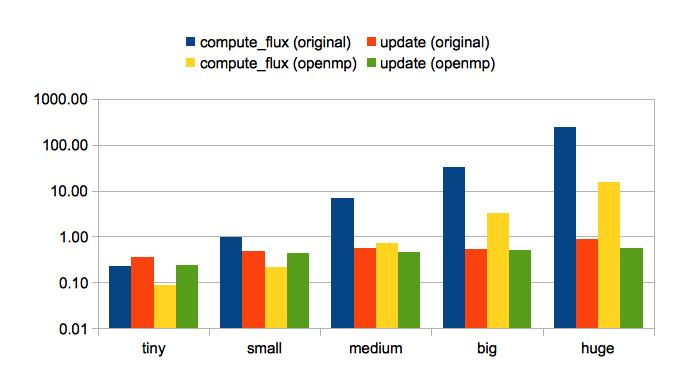
\includegraphics[width=\columnwidth]{images/omp_orig.jpg}
	\end{center}
	\caption{Comparative execution times for the original code and the OpenMP version. (log scale)}
	\label{fig:ompvsorig}
\end{figure}

Using the Amdahl's Law, one can calculate the maximum achievable speedup, thus finding the limits of parallelization in an application's performance.

$$\mathrm{speedup_{max}}=\frac{1}{s+\frac{p}{N}}$$

Being $N=24$ the number of parallel hardware threads, and $p=0.94$ the parallel fraction of the code (see \autoref{sec:initprof}),
\begin{IEEEeqnarray}{CrClC}
& \mathrm{speedup_{max}} & = & \frac{1}{(1 - 0.94) + \frac{0.94}{24}} & \Leftrightarrow	\nonumber \\
\Leftrightarrow & \mathrm{speedup_{max}} & = & 10.08 \enspace .
\end{IEEEeqnarray}

Calculating the speedup obtained from the parallelization alone:
\begin{IEEEeqnarray}{CrClC}
& \frac{8.33}{3.37} & = & 2.47
\end{IEEEeqnarray}
which shows that only 25\% of the possible speedup was achieved even after all these optimizations.

\section{CUDA}
\label{sec:cuda}

\subsection{Implementation}

Unlike the OpenMP implementation, which could operate on the existing data structures (although not as efficiently as it would with the optimized structures), for a CUDA implementation a different approach was required from the start. As it was already stated, the original FVLib implementation relied heavily on dereferencing, which not only increases the number of memory accesses, but also spreads data in a non sequential way in memory. This is an even bigger problem in a GPU, which requires memory accesses to be as efficient as possible, in order to take full advantage of the hardware.\\
Besides, copying all data to GPU memory would also be a difficult task. Since data is not in a single sequential block, multiple copy operations would be required.\\

\subsubsection{Data Structures}

The first step towards the CUDA implementation of the algorithm was rewriting the data structures. It was also a chance to organize data in a more efficient way. GPUs store data interleaved in different memory banks, and multiple accesses to different banks can be done in parallel, with no overhead. This is one of the reasons that make GPUs work better with data structures in the form of a Struct-of-arrays, instead of Array-of-structs, which are the most intuitive, but also more widely used for CPU implementations.\\

\subsubsection{Kernels}

While the OpenMP version only required \texttt{compute\_flux} function to be paralellized in order the see a speed-up, this is not true in CUDA. If only a portion of the main loop is replaced with CUDA code, in this case \texttt{compute\_flux}, then two memory transactions would be required every iteration, one to copy the calculated flux from the GPU to compute the rest of the loop, and later the new polution values would have to be copied again back to the GPU for the next iteration. This overhead was noticed on the first tests, after implementing \texttt{compute\_flux}. Although no actual measurements were made, this partial CUDA version was clearly much slower than the original, sequential version. So the last step was to parallelize the rest of the main loop.\\

A second implementation was made, implementing the kernels for the rest of the main loop. The \texttt{reduction} was based on the highly optimized example from the NVidia CUDA Samples. It is obviously much different from the original code, but since reduction is a common base example in CUDA, it's implementation is already deeply studied. The only problem with the current implementation is the fact that it is not fully executed in GPU. Currently, the GPU is computing the reduction per-block, where each block returns the reduced value from it's share of the array. The final array (which is extremelly smaller than the total amount of values) is then copied back to the CPU, where the final reduction takes place.\\

About the \texttt{update}, it was already explained in \autoref{subsec:dependencies} that this function suffers from a data race between iterations, so it had to be rewritten, to iterate through the cells, instead of the edges. The final implementation was tested to assert that it was producing the same outputs as the original function. This was true to a certain extent. Due to the fact that the operations were being done in a different order, some precision differences were noticed due to floating point limitations. However, the magnitude of these differences was small, and as it was confirmed with Prof. Stéphane, were not important.\\

The final step of the main loop is where the current polution file is written to the output file after a certain number of iterations, creating an animation of the polution spreading. Since this option was discarded at the beggining of the project, it was not being used here, and thus was not the focus when analysing performance. The code however, will require changes in order to remove (or at least reduce) the bottleneck created by the output functions.\\

Both the \texttt{compute\_flux} and the \texttt{update} kernels are extremely naive, since they were implemented based on the original algorithms. The initial objective was to simply perform the same operations without compromising readability of the code. Future work will include a deeper analysis of this kernels in an attempt to find out whether an optimization is possible (or useful).

\subsubsection{Optimization}

There was not much effort in optimizing the code once it was working properly. However, as mentioned in \autoref{subsec:dependencies}, the removal of the reduction from the main loop, due to it being constant along the entire program, was an optimization that could be achieved with little programming effort, and gave a considerable performance gain, especially with smaller inputs, as it will be shown in the next section.\\

Another easy point of optimization was the optimal selection of the number of blocks and threads for each kernel. This was done with the help of the Cuda Occupancy Calculator \cite{calculator}. This spreadsheet was created by NVidia to assist developers in selecting the optimal grind a block size for each kernel. By either compiling the code with specific flags, or by checking profiler information, it is possible to know the amount of registers and shared memory the compiler has selected for each thread, and with that information, the spreadsheet can give the optimal number of threads per block to achieve better occupancy of each Streaming Multiprocessor, thus making better use of the hardware.

\subsection{Profiling Methodology}

\subsubsection{Testing Environment}

For all tests, SeARCH node 511-1 was used. This node was already characterized in \autoref{subsubsec:env}, except for it's CUDA device:

\begin{itemize}
	\item 2x NVidia Tesla C2050 (only one was used)
	\begin{itemize}
		\item 448 CUDA Cores @ 1.15 GHz
		\item 3GB GDDR5 @ 1.5 GHz
		\item 515 GFlops max. (with double precision)
	\end{itemize}
\end{itemize}

This was the only available environment to test the application, as double precision floating point support is only available since CUDA 1.3, which is not supported in the other GPUs at the SeARCH cluster. Because of that, it was impossible to deliver a comparative analysis of the application in different CUDA devices.

\subsubsection{Profiler}

Two profiling methods were used. CUDA Events provide a simple way to measure time elapsed in a segment of code. Also, the CUDA Profiler enables a set of hardware counters to retrieve information about certain events.
Although both tools were used, CUDA Profiler counters were not of much use, since the values they measure are only intended for GPU vs GPU comparison (as stated by it's manual), to understand the impact of optimizations in the code. They do not provide relevant data to compare against a CPU implementation. Profiler data was still collected though, and will probably be useful for future work with the library.

\subsubsection{Test Cases}

The test cases used are the same of the previous implementations, and are detailed in \autoref{subsubsec:testcases}.

\subsection{Results}

The following data is based on the timestamps extracted from the algorithm with CUDA Events API. All graphs are in logarithmic scale, and represent events for all five of the previously mentioned test cases.

\subsubsection{Kernel Execution Time}

In \autoref{fig:cuda_kernels} it can be seen that, for this implementation, \texttt{compute\_flux} and \texttt{update} are the fastest kernels in the smaller cases, but their execution time also increases faster as the mesh size increases. The reduction on the other hand, seems to be the bottleneck, but this is not true for bigger meshes. This is because of the fact that the reduction is implemented with the help of the NVidia samples, which resulted in a highly optimized kernel, while both \texttt{compute\_flux} and \texttt{update} were both written from scratch and still require a more intelligent approach (for instance, shared memory was not used, and should increase the performance significantly).

\begin{figure}[!htp]
	\begin{center}
		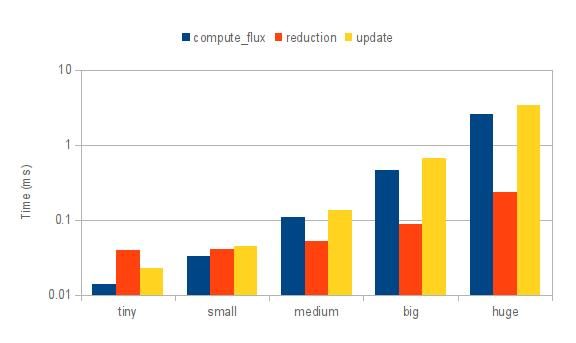
\includegraphics[width=\columnwidth]{images/report/cuda_1_kernels}
	\end{center}
	\caption{Kernel execution time \label{fig:cuda_kernels}}
\end{figure}

\autoref{fig:cuda_kernels_opt} shows the same information, but for the optimized version of the algorithm, where the reduction was removed. Since most of the calculations for the array to be reduced were done in \texttt{compute\_flux}, it's execution time naturally decreased, making \texttt{update} the most expensive for this version.

\begin{figure}[!hpt]
	\begin{center}
		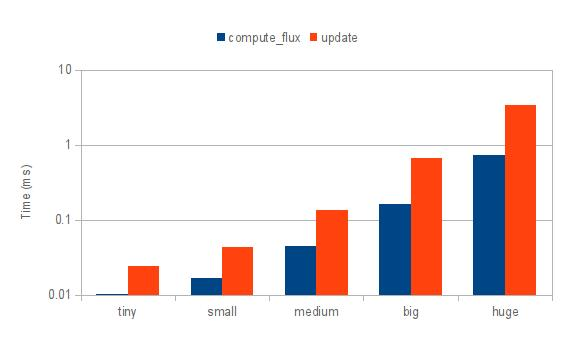
\includegraphics[width=\columnwidth]{images/report/cuda_3_kernels_opt}
	\end{center}
	\caption{Kernel execution time (after reduction removal) \label{fig:cuda_kernels_opt}}
\end{figure}

\subsubsection{Total Program Time}

\autoref{fig:comp_all} shows the global execution time for all versions of the implementation. About the two CUDA implementations (with and without the reduction), it can be noted that for the smaller cases, there is pratically no difference between the first version and the optimized one. The biggest test case however, shows a performance increase around 25\%. This can be explained due to the fact that, even though the reduction kernel, by itself, is not the bottleneck, it's implementation required a small amount of memory to be copied from the GPU to the CPU every iteration. That was most likely a big bottleneck for the loop, since the GPU could not advance it's work while the transaction, and the subsequent end of the reduction, was finished, since it depended on it's final result. So the removal of this processo actually shows a significant improvement, although this can only be seen for bigger inputs.

\section{Comparative Analysiys}
\label{sec:comparison}

A final analysis of the execution time was made between the original sequential code and all the implemented versions of the algorithm. Original refers to the unaltered, sequential version. The following four versions correspond to incremental changes of the original implementation, respectively with better data structures, following the preparation of the \texttt{update} function for parallelization, and then the Optimal version, where the need for a reduction was removed from the main loop.\\

The CUDA implementations correspond to the initial version, with the three kernels implemented, following the optimized version, where the reduction was optimized out of the loop.

\begin{figure}[!hpt]
	\begin{center}
		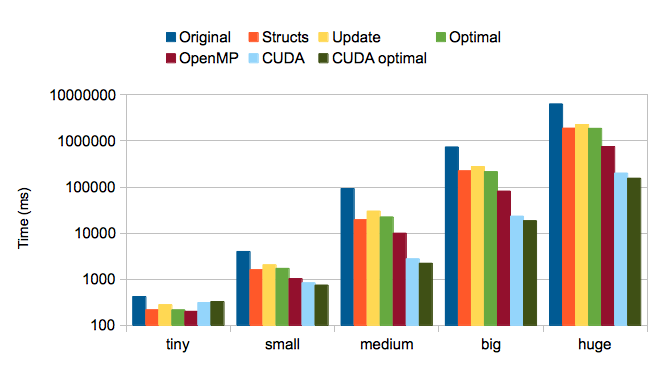
\includegraphics[width=\columnwidth]{images/comp_all}
	\end{center}
	\caption{Total program time (comparison) \label{fig:comp_all}}
\end{figure}

The tests named Structs, Update and Optimal are only meant to provide an incremental analysis of the work done with the CPU implementation. OpenMP was only added after some previous work was done with the code, to remove dependencies and optimize sequential performance.\\
For the smallest test case, the OpenMP version gives the best result, while the optimized CUDA version provides lower execution times for the rest of the tests. The result for the tiny test is different because the CUDA version has a bigger overhead, since it needs to copy all the data structures to the device, and probably perform some initialization of the CUDA driver. This overhead, although small, is enough to be significant in this small test case.

\section{Conclusion}
\label{sec:conclusion}
In this document was described the analysis, optimization and parallelization process of a scientific application to simulate the spread of a pollutant in a given space through time, as well as a quantitive profile of both original and developed code.

The primary analysis showed some obvious problems with the original implementation, related with memory access, inefficient programming practices and not explored simplifications. This first review also provided a clear image of the problem, allowing the identification of the two major parallelization candidates -- \texttt{compute\_flux} and \texttt{update}.

The discovered problems were studied and solved, greatly improving the application's code due to the implementation of new data structures and by removing the preparations for features that were not implemented in the original. Also, the complete parallelization of all the identified targets was made possible by removing parallelization obstacles such as dependences. This was achieved with a deep analysis of the \texttt{compute\_flux} function and by changing how \texttt{update} iterated the space.

Two parallel optimized versions of the application were implemented: one in shared memory using OpenMP; another in GPU using CUDA. The first, was built incrementally from the original application, implementing a modification or optimization at a time. The second, due to it's different nature, has it's core redesigned almost from scratch to meet the different hardware.

A formal profiling was performed for each of the parallel versions, mainly based in execution times. For the OpenMP version, the analysis of the collected data was mainly focused in comparing the impact of the performed modifications in the original code, towards showing which steps were more significant to a performance improvement. The analysis of the data collected with the CUDA implementation was compared with all the CPU implementations, thus forming a clearer picture of which scales better.

The OpenMP implementation showed very high speedups when compared to the original code, due to the optimizations performed. Yet, it also showed that, despite being parallelized, the \texttt{update} function did not show as high speedups as the \texttt{compute\_flux}. Since the only significant improvement in this function came from the new data structures, this behavior shows a clear bottleneck in memory communication.

While the overhead involved with the GPU hardware prevented the CUDA version from achieving the best results in the smallest test cases, as the data size increases and this overhead becomes less significant, the GPU implementation clearly achieves constant better results than any CPU version, including the parallel version with OpenMP. Consequently, the GPU version is the best approach to a high performance scalable code.

\subsection{Future Work}

% Para OMP
The performed optimizations striped the original code from all the obvious bottlenecks even before parallelization. Yet, as demonstrated in \autoref{sec:omp:results} the OpenMP version can still be target of improvements.\\

The first improvement would be directly related with FVLib. While most of it's impact are out of the application, it is still used as an intermediary between the saved data and the computation. This can decrease a starting overhead and allow the application to start faster.

However, improving anything outside the main loop will have little effect on larger test cases, as the fraction of time spent in preparations will be increasingly small. The main target of any future performance improvement must be the \texttt{update} function, either by exploring other cache-friendly approaches, methods to improve locality and, as stated before in this document, by removing problems such as false-sharing.

% Para CUDA
For the CUDA version, one of the first tasks that is required, is to remove the dependency from the original data structures, by implementing direct I/O methods. Currently, data is read to the original structures in FVLib, and only then translated to the new ones, creating an unnecessary overhead.\\

The kernels also require some extra work, in order to increase their speed and reduce the overhead of their calls. To reduce the overhead, the usage of streams might give good results. For better performance, the kernels themselves may be optimized, not only the code itself, but also by taking advantage of shared memory.

% Em geral
Overall, for all versions of the algorithm, there should also be some work about the animation implementation, by studying efficient ways to allow the animation to be saved every few iterations, without creating the huge bottleneck that was seen on the initial analysis. It does not matter how much optimized the CUDA or OpenMP code is: if an animation is required as output, then it will always be the bottleneck in the current versions. New approaches should be studied to optimize this process, and prevent the output from delaying the whole algorithm.


%\label{sec:cuda}
%\subsection{Data Structures}
%For a GPU implementation, all the data structures had to be converted to a suitable format (using sequential memory positions instead of dereferencing). Since this was required from the start, it was also a chance to optimize memory for GPU computing, by using a structure of arrays instead of an array of structures, to take advantage of the GPU's coallesced memory accesses.
%
%\subsection{Implementation}
%
%
%\subsubsection{Flux Computation}
%A total of 3 CUDA kernels were written for the implementation. The first one was to replace the \texttt{compute\_flux} function. This is a very straight-forward implementation, with no major changes to the original algorithm, aside from the fact that each CUDA thread handles a single element, instead of looping through the mesh.
%
%%\paragraphh{\texttt{max} reduction}
%%As previously explained, a reduction calculation was also required to allow for parallelization of the \texttt{compute\_flux} function. This is a widely used example in CUDA, and was implemented with the help of the NVidia samples.
%
%\subsubsection{Mesh Update}
%The \texttt{update} function was also converted to CUDA. This was not as interesting to parallelize in the OpenMP version, since it doesn't occupy the majority of the time. However, using the original CPU implementation would mean that for every iteration of the main loop, flux and polution data had to be copied back from the GPU to execute the update, and then copied again to GPU for the next iteration. This would eliminate any advantage of GPU parallelization, so this function had to be re-written, taking into consideration the data races of the original one.
%
%\section{Conclusion}
%In this document the original application code was analyzed and studied. The two key functions in the program execution were identified using the program's callgraph. Also, a major bottleneck was identified in the animation generation, which invalidated any computation optimization effort when activated.
%
%Several problems were easily detected in early stages, along with parallelization obstacles. These problems were mostly related with the program's memory usage, and some even prevented parallelization. The identified obstacles, namely data dependences, were solved by manipulating the original code, only possible due to an increasingly better understanding of the algorithm. 
%
%Two parallel versions of the application were implemented. The first version implemented the same code using the OpenMP directives to parallelize the most critical part of the program. The second version adapted the original code to perform all the required computations in a GPU using CUDA.
%
%All versions still lack a formal profiling which would allow to identify bottlenecks and compare efficiency. Despite that, both of the implemented parallel versions showed a small but consistent speedup in multiple executions. While this shows that the application can be improved with parallelization, the differences classify the algorithm as non-scalable.
%
%Further optimization efforts can be done to improve the obtained results. For the OpenMP implementation, these include extending the parallelization to the \texttt{update} function and changing the data structures. For the CUDA implementation, a revision of memory access efficency might be useful, as well as the usage of CUDA Streams to minimize idle time of the GPU. Also, for both implementations, changing how the FVLib library works, specifically how the data is accessed, could greatly improve the program efficiency specially with the animation generation.


%	Side Notes: OpenFVM.sourceforge.net

\begin{thebibliography}{12345}

%\bibitem[FVM]{finite}
%	Joaquim Peiró and Spencer Sherwin	\\
%	\textit{Finite Difference, Finite Element and Finite Volume Methods for Partial Differential Equations}	\\
%	Department of Aeronautics, Imperial College, London, UK	\\
%	\texttt{\smaller http://multiscale.emsl.pnl.gov/docs/finite.pdf}

\bibitem[OMP]{openmp}
	\textit{OpenMP Application Program Interface}	\\
	OpenMP Architecture Review Board	\\
	Version 3.1, July 2011

\bibitem[NVIDIA]{nvidia}
	\hfill\\
	\texttt{\smaller http://developer.nvidia.com/category/zone/cuda-zone}
	
\bibitem[AMD6100]{AMD6100}
	\textit{The AMD Opteron™ processor is the ideal solution for High Performance Computing}\\
	AMD Documents\\
	\texttt{\smaller http://sites.amd.com/us/Documents/\\AMD\_Opteron\_ideal\_for\_HPC.pdf}

% TODO corrigir este
\bibitem[CUDA By Example]{cudabook}
	Jason Sanders, Edward Kandrot	\\
	\textit{CUDA By Example: An Introduction to General-Purpose GPU Programming}

\bibitem[CUDA Profiler]{profiler}
	\hfill\\
	\texttt{\smaller http://developer.download.nvidia.com/compute/cuda/3\_0\\/toolkit/docs/visual\_profiler\_cuda/CUDA\_Profiler\_3.0.txt}

\bibitem[CUDA Occupancy Calculator]{calculator}
	\hfill\\
	\texttt{http://developer.download.nvidia.com\\/compute/cuda/CUDA\_Occupancy\_calculator.xls}
\end{thebibliography}

\end{document}
